\section{Experiment}
\label{sec:experiment}
We propose the CSGANs framework, which translate images from one domain to another, being able to capture long range dependencies and reserve the global structures. To demonstrate the effectiveness of our framework, we have performed several experiments. In this section, we discuss 
\subsection{Implementation Details}
In order to comparing with the pix2pix model, we basically follow its implementation details. We use minibatch SGD and Adam \cite{Adam} optimizer with learning rate $lr=0.002$ and momentum parameters $\beta_1=0.5, \beta_2=0.999$. We update one step for either of $G$ and $D$ alternatively. Batch normalization is used in convolutional layers of the generator. Batch size is set to 8.
\subsection{Dataset}
We evaluation our method with the task of translating edge maps to natural images, e.g. the target images are face images while the conditional images are the corresponding edge maps. The face images of the dataset we used are face images of CelebA dataset \cite{CelebA}, which  is a large-scale face attributes dataset with more than 200K celebrity images. Faces have well-defined structure of eyes, noses, mouths, and etc., and therefore the artifacts are visually sensitive for observers. This makes face images suitable for evaluating the proposed method.  We utilize the cropped and aligned version of dataset with the size of every images being $218\times 178$. In order to meat the original setting of the pix2pix method, we center-crop the images and resize the image to $256\times 256$ in both experiments of the pix2pix model and the proposed model. The face attributes are attached in the dataset but not included in our experiments. 

The edge maps we use generated in the pipeline similar to that used in pix2pix paper. Specifically, the edges are firstly extracted using a deep edge detector named holistically-nested edge detect (HED) \cite{HED}. We keep the values of each edge pixels calculated by HED in the edge maps. Each of these values is supposed to indicate the probability of being edge in the positions of pixel. And then several steps of post-processing are conducted to obtain simpler and clearer edge maps with fewer edge fragments, including thinning, short edge removal, and erosion. In addition, since the edge maps are very sparse, we add one more step to the process to decrease the sparsity of edge maps. We calculate an unsigned euclidean distance field for each edge map to obtain a dense representation. We note that similar idea of distance filed representations can be found in some recent works \cite{repair_3d, shape_completion, SketchyGANs}. In Section \ref{subsec:ablation}, we will prove the advantages of distance fields by experiments.

%
%
\subsection{ Evaluation Metrics}
The evaluation of generative models is an open and complicated task, because a model with good performance with respect to one criterion need not imply good performances with respect to the other criteria \cite{evaluation, GANs_equal}. Traditional metrics, such as pixel-wise mean-squared error do not present the joint statistics of the synthesized samples and therefore is not able to evaluation the performance to a conditional generated model. 
Inception Score (IS) \cite{IS} is a widely-used criterion. However, IS has been pointed out to have serious limitations that it focuses more on the recognizability of the generated images rather than realism of details or intra-class diversity \cite{evaluation}. Moreover, IS is an evaluation metric for class-aware task which is not suitable for our experiments.
 
Since the goal of image-to-image translation is to generate from the conditional image an corresponding image visually plausible to human, we mainly compare the results between different models by perceptual user studies. Several related works have proposed similar perceptual experiments \cite{LaplaceGANs, SRGANs, Improved_techniques, CRN, pix2pixHD}. Following the similar procedure as described in \cite{CRN}, we conduct two different kinds of experiments: unlimited time user study and limited time user study. 
In addition, we use anther popular criterion, Fr\'echet Inception Distance (FID) \cite{FID}, to prove the effectiveness of proposed method quantitatively. More details are explained below.
\paragraph{Unlimited Time User Study}
% with/without the option "equally well"
% present the images in one second or in unlimited time (select in unlimited time)
% two setting: unlimited time=>which one is better, limited time=>how long to find the advantage of the proposed method
We utilize perceptual user study experiments to compare the generated samples between different models. In every trial, we randomly select a conditional image from the testing dataset and generate two synthesized images from pix2pix and our model that are going to be compared with each other. These three images are displayed side by side, and the user is asked to pick one from the two synthesized images within unlimited time based on "which is more realistic and matches the conditional image better". The options offered to users are two of the synthesized images. No feedback is provided after every trial to avoid misguiding the user's perceptual judgment and preference. 00 users participate this experiments, and 00 trials are provided to every user.
>>>>> Discuss the results <<<<<<<< 
\paragraph{Limited Time User Study}
For this task, we evaluates how quickly the users can perceive the differences between images. In every comparison, we  select three images corresponding to one randomly drawn edge maps (two generated by pix2pix and our model, and the ground truth). Similarly, two of these three images are displayed to the use with the edge map side by side for a short period of time. The user is asked to pick one of two displayed face images also based on "which is more realistic and matches the conditional image better". The duration is randomly selected between $1/8$ seconds and $8$ seconds. 
\paragraph{Fr\'echet Inception Distance (FID)}
Fr\'echet Inception Distance (FID) \cite{FID} is a recently proposed and widely used evaluation metric for generative models, which is shown to be consistent with human perceptual evaluation in assessing the realism and variation of generated samples. FID uses an Inception network to extract features and calculates the Wasserstein-2 distance between features of the generated images and the real images. Models with lower FID values are supposed to model a synthetic distribution closer to the real distribution. We inference each model with the conditional images in the testing set to get the generated samples, and calculate the FID with respect to the target images in the testing set.
%
%
\subsection{Comparison with pix2pix}
%
% TODO: finish this section after finishing the experiments
In this section, experiments are conducted to compare the images generated by the pix2pix model and the proposed model. The comparisons are describe blow.
\paragraph{User Study} Two kinds of user studies are performed.The unlimited time user study is designed to evaluate the perceptual quality of the generated image, the results of which are shown in Table \ref{table:unlimited_time}. We can observe that ....The limited time user studies are designed to evaluate how quickly the users cn perceive the differences between images. Figure \ref{fig:limited_time} shows the results......
\paragraph{MS-SSIM and FID} xxxx
%
%
\begin{table}[h]
	\centering	
	\label{tab:evaluation_metrics}
	\caption{Evaluation metrics }
	\begin{tabular}{|l|c|c|}\hline
		Generated Images & MS-SSIM & FID\\\hline
		Dataset & $0$ & $0$\\
		pix2pix & $0$ & $0$ \\
		-Distance fields & $0$ & $0$\\
		-Spetral Normalization & $0$ & $0$\\
		-Global Discriminator & $0$ & $0$ \\
		-Conditional Connection & $0$ & $0$ \\
		Full model & $0$ & $0$ \\\hline
	\end{tabular}
\end{table}
%
%
\begin{figure}
	\label{fig:results}
	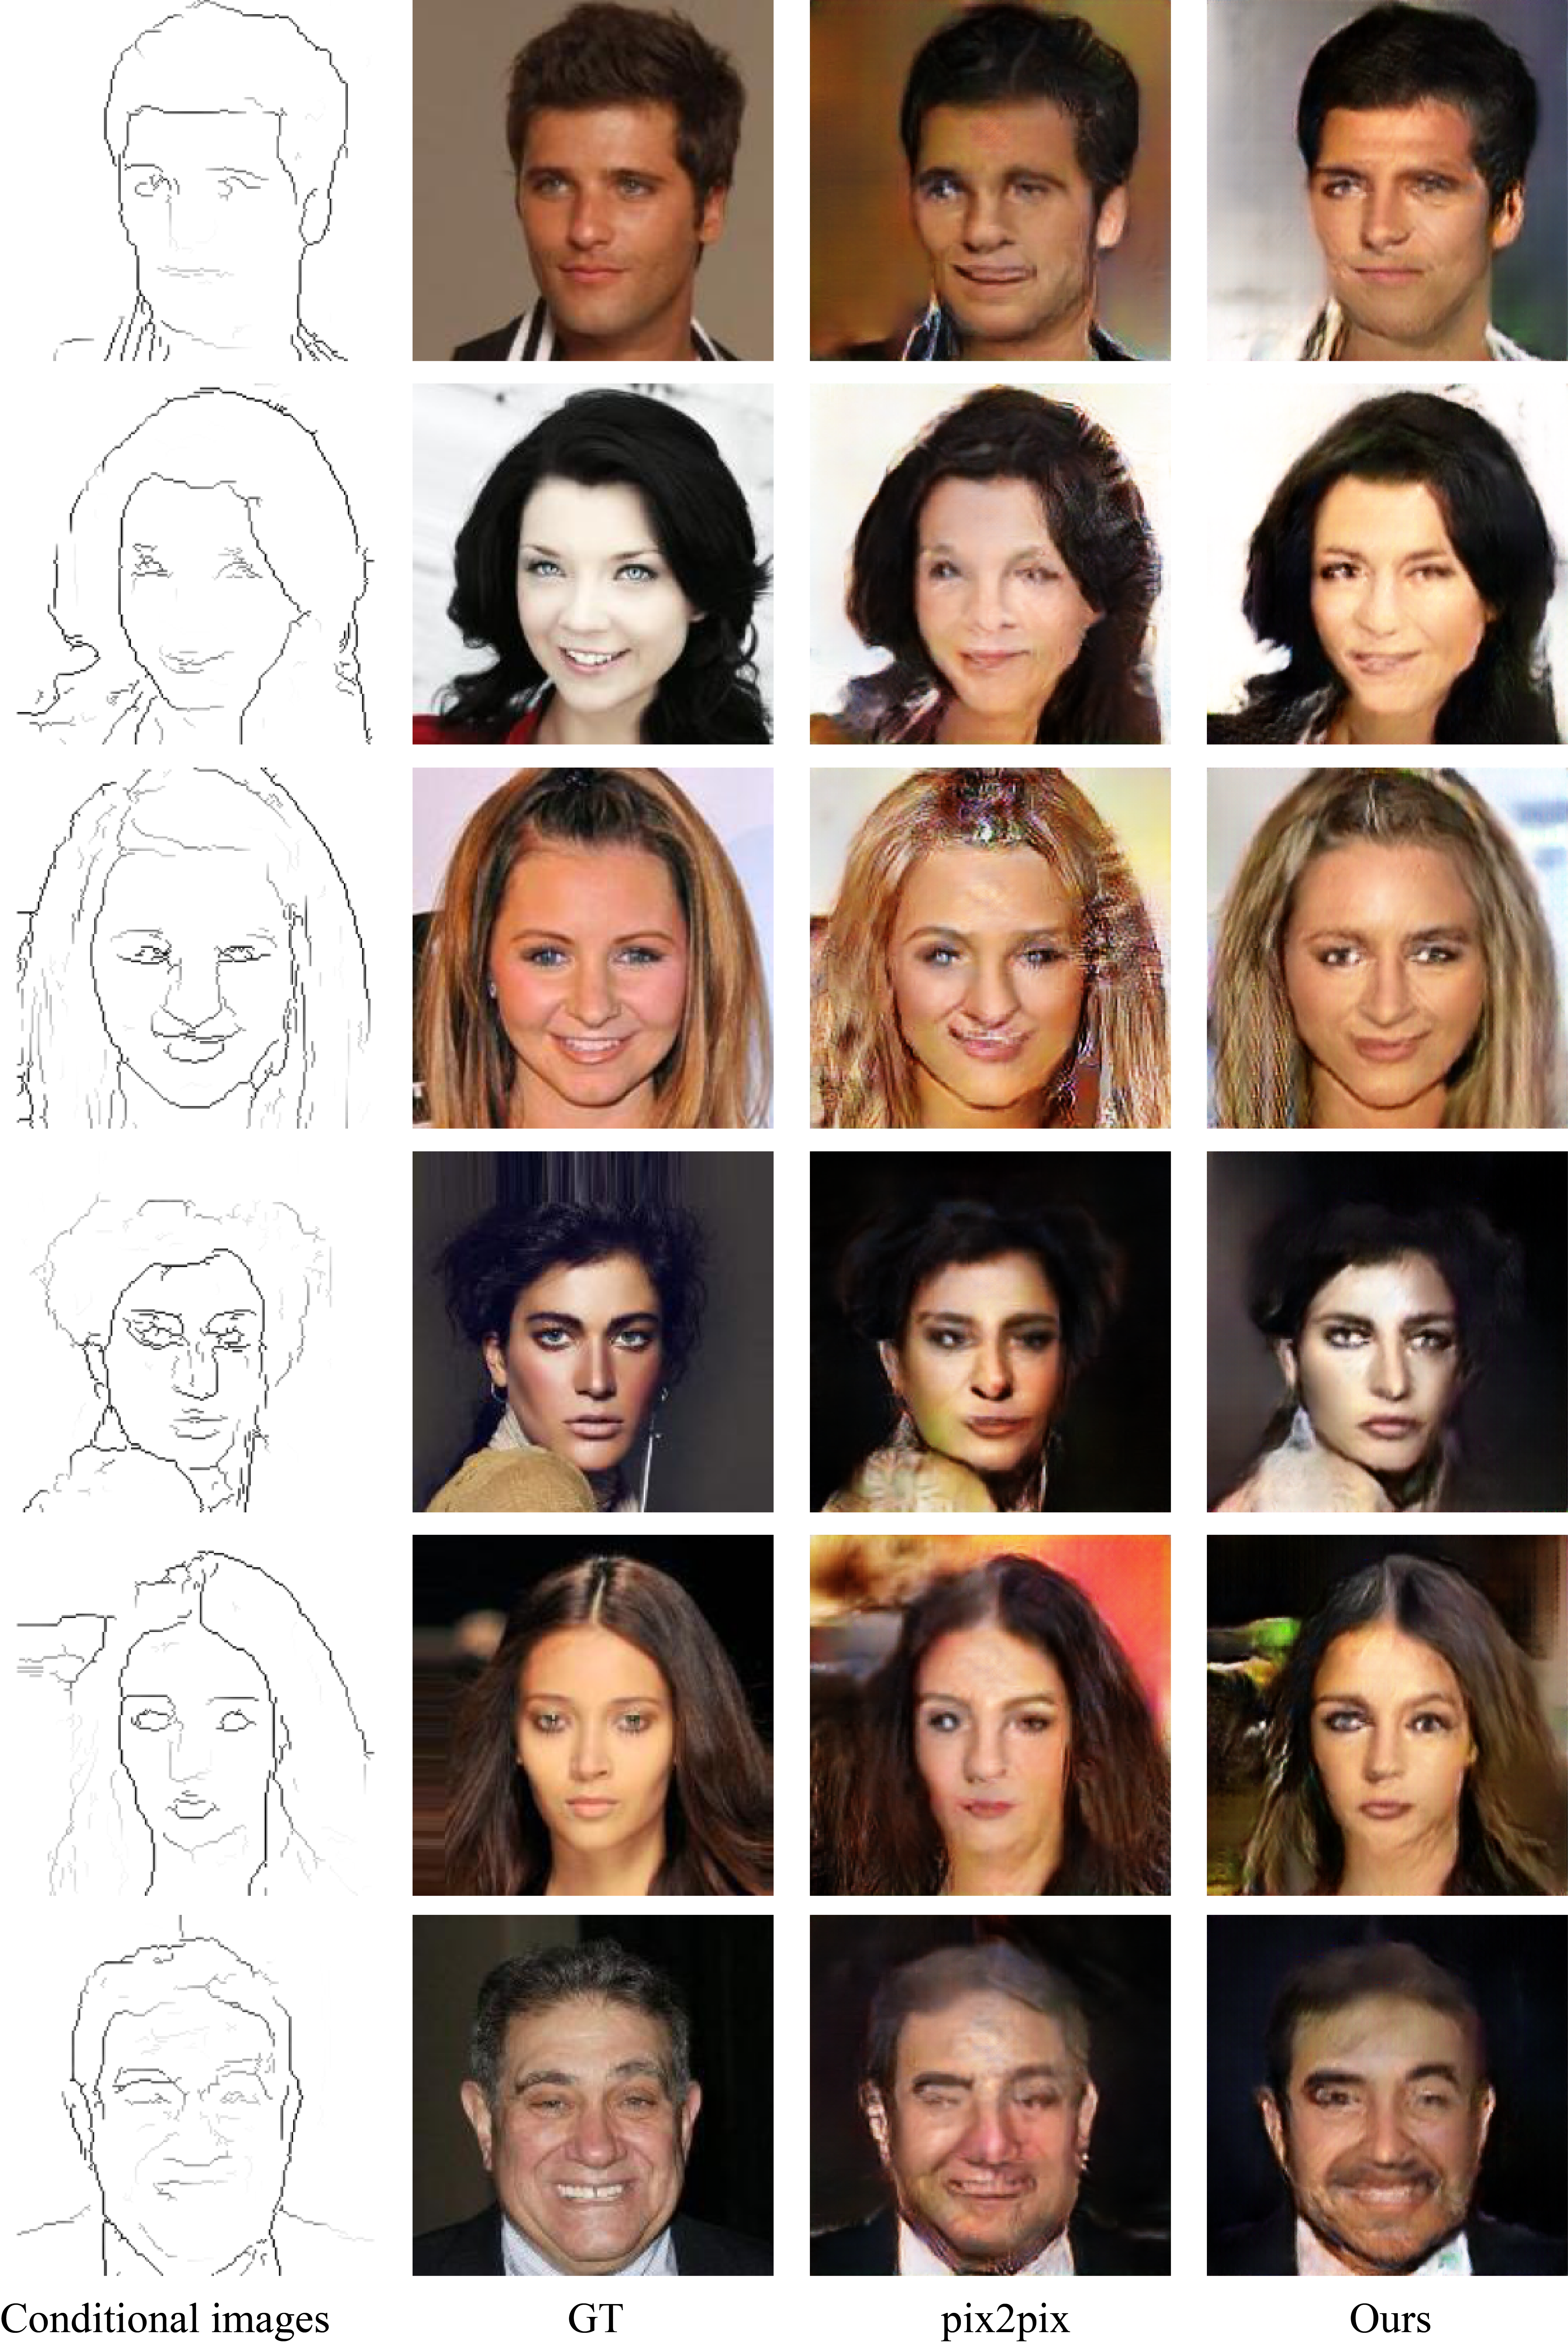
\includegraphics[width=0.8\textwidth]{figures/results}
	\caption{results}
\end{figure}
%
%
\subsection{Ablation study}
